\documentclass{beamer}

\usepackage[utf8]{inputenc}
\usepackage[english]{babel}

\usepackage{amsmath}
\usepackage{nicefrac}

\usepackage{minted}
\usepackage{fontspec}

\usepackage{xcolor}
\usepackage{graphicx}

\usemintedstyle{friendly}
\setmonofont{Source Code Pro}
\usetheme{metropolis}

\newminted{rust}{escapeinside=||, fontsize=\footnotesize, bgcolor=bg, autogobble, rust}
\newminted{java}{escapeinside=||, fontsize=\footnotesize, bgcolor=bg, autogobble, java}

\newcommand{\then}{\Rightarrow}
\newcommand{\code}[1] {\texttt{\footnotesize #1}}

\title{Bounded generics over constants in Rust}
\author{Author: Christian Poveda \\ Advisor: Nicolás Cardozo}
\institute{Systems and Computing Engineering Department \\ Universidad de los Andes \\ 
\includegraphics[width=3cm]{./flag.png}}
\date{2018-09-18}

\begin{document}

\frame{\titlepage}

\begin{frame}[fragile]
    \frametitle{Context: What is a type?}
    On this snippet
    \begin{javacode}
        String myString = "Hello, World!";
    \end{javacode}
    \code{String} is the type of \code{myString} and as such, it determines:
    \begin{itemize}
        \item The operations on which \code{myString} could be used.
        \item The values \code{myString} could take.
        \item The type of \code{"Hello, World!"} (it should be \code{String}).
    \end{itemize}
    To be more general: 
    \begin{center}
        \textit{A type system is a syntatic method for proving the absence of certain program behaviors by classifying phrases according to the kinds of values they compute}
    \end{center}
\end{frame}

\begin{frame}[fragile]
    \frametitle{Context: The Rust programming language}
    Rust is a systems programming language focused on safety, speed and concurrency. It is sponsored by Mozilla. 
    
    However, Rust is not your typical language:
    \begin{itemize}
        \item It does not have garbage collection nor pointer arithmetic, but it is memory safe.
        \item It is blazingly fast (as fast as C++), but it has high-level features:
            \begin{itemize}
                \item Pattern matching
                \item Traits
                \item Higher order functions
            \end{itemize}
        \item It features concurrency without data races.
    \end{itemize}
\end{frame}

\begin{frame}[fragile]
    \frametitle{Context: Rust's type system}
    Rust's type system is based on the ML type system. As such it has:
    \begin{itemize}
        \item Static type checking (i.e., programs are checked for safety during compilation).
        \item Type inference (i.e., type annotations are not always needed).
        \item Polymorphism via traits and generics.
        \item Enums and Structs.
    \end{itemize}
    It also takes care of memory safety
    \begin{itemize}
        \item Rust encodes the lifetime of each variable in its type.
        \item For each variable, Rust only allows one of the following:
            \begin{itemize}
                \item One mutable reference.
                \item Several inmutable references.
            \end{itemize}
    \end{itemize}
\end{frame}

\begin{frame}[fragile]
    \frametitle{The problem: Functions over arrays}
    In Rust, Arrays (being stack allocated) must be statically sized.

    As a consequence, this code compiles
    \begin{rustcode}
    fn add_arr(a: &[f64; 3], b: &[f64; 3]) -> [f64; 3] {
        let mut result = [0.0; 3];
        for i in 0..3 {
            result[i] = a[i] + b[i];
        }
        result
    }
    \end{rustcode}
\end{frame}

\begin{frame}[fragile]
    \frametitle{The problem: Functions over arrays}
    In Rust, Arrays (being stack allocated) must be statically sized.

    But this code does not
    \begin{rustcode}
    fn add_arr(a: &[f64; N], b: &[f64; N]) -> [f64; N] {
        let mut result = [0.0; N];
        for i in 0..N {
            result[i] = a[i] + b[i];
        }
        result
    }
    \end{rustcode}
\end{frame}

\begin{frame}[fragile]
    \frametitle{The solution: Generics over constants}
    Generics are a way of archieving polymorphism based on parametrizing types. For example
    \begin{itemize}
        \item \code{Vec<T>} is the type of vectors of elements of type T
        \item \code{Vec<bool>} is the type of vectors of booleans
        \item \code{Vec<i32>} is the type of vectors of integers
    \end{itemize}
    We could allow the same pattern letting constant values be parameters
    \begin{itemize}
        \item \code{[bool; N]} is the type of arrays of booleans and size N 
        \item \code{[bool; 0]} is the type of arrays of booleans and size 0 
        \item \code{[bool; 1]} is the type of arrays of booleans and size 1
    \end{itemize}
    We only use constants because Rust's type checking is static.
\end{frame}

\begin{frame}[fragile]
    \frametitle{The solution: Generics over constants}
    In general, a type \code{Foo} parametrized by a constant \code{C} of type \code{T} would be written as
    \begin{rustcode}
        Foo<const C: T>
    \end{rustcode}
    In a similar fashion, a function \code{bar} parametrized by a constant \code{C} of type \code{T} would be written as
    \begin{rustcode}
        fn bar<const C: T> (args) -> ReturnType { ... }
    \end{rustcode}
    Is important to say that the dispatch mechanism in Rust is static. 
    
    On compilation, generic functions and generic types are specialized on demand.
\end{frame}

\begin{frame}[fragile]
    \frametitle{The solution: Arrays as const-generic types}
    With generics over constant values, we can write traits and functions for any array size
    \begin{rustcode}
    fn add_arr<const N: usize> (a: &[f64; N], b: &[f64; N]) 
    -> [f64; N] {
            let mut result = [0.0; N];
        for i in 0..N {
            result[i] = a[i] + b[i];
        }
        result
    }
    \end{rustcode}
    However, this is only a partial solution...
\end{frame}

\begin{frame}[fragile]
    \frametitle{The problem: Dynamical check of static bounds}
    Consider the following generic function
    \begin{rustcode}
        fn <const N: usize> head(a: [f64; N]) -> Option<f64> {
            if N > 0 {
                Some(a[0])
            } else {
                None
            }
        }
    \end{rustcode}
    The restriction \code{N > 0} is checked at runtime even though \code{N} will not change after compilation
\end{frame}

\begin{frame}[fragile]
    \frametitle{The solution: Bounded generics over constant values}
    Given that now constants are valid parameters. Rust's type checker could take care of checking properties over them.

    If \code{P: bool} is a boolean expression depending on a constant \code{C}, we can restrict \code{C} as a parameter
    \begin{rustcode}
        // A generic type over a bounded constant
        Foo<const C: T> with P
        // A generic function over a bounded constant
        fn bar<const C: T> (args) -> ReturnType with P { ... }
    \end{rustcode}

    Now, the type checker enforces that any instance of \code{Foo} and \code{bar} over a constant satisfies \code{P}
    
\end{frame}

\begin{frame}[fragile]
    \frametitle{The solution: Statical check of static bounds}
    Now, we can write static bounds over constant parameters.
    \begin{rustcode}
        fn <const N: usize> head(a: [f64; N]) with {N > 0} -> f64 {
            a[0]
        }
    \end{rustcode}
    Given that the bound \code{N > 0} is checked during compilation and not in runtime, this code is not just shorter, it is also faster.
\end{frame}

\begin{frame}[fragile]
    \frametitle{Related work: Generics over values in theory}
    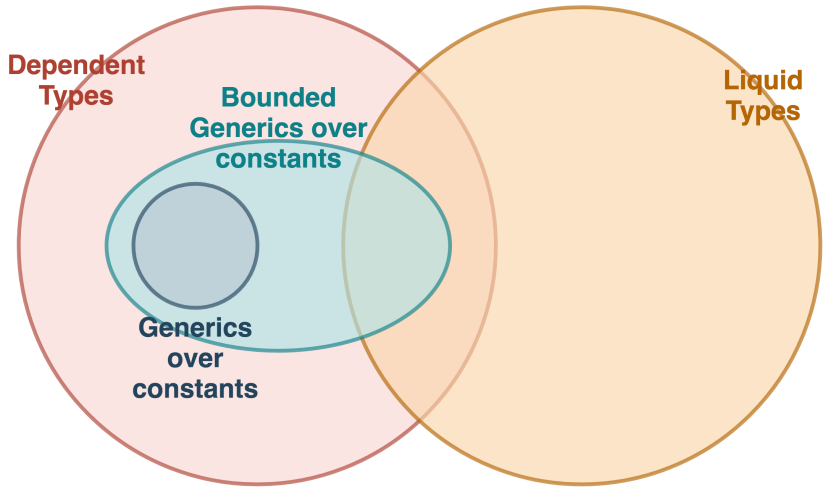
\includegraphics[width=\textwidth]{./theory.png}
\end{frame}

\begin{frame}[fragile]
    \frametitle{Related work: Languages with dependent types}
\end{frame}

\begin{frame}[fragile]
    \frametitle{Related work: Rust Status Quo}
    The Rust community is already working on an implementation of generics over constants. However, this implementation still needs:
    \begin{itemize}
        \item A mechanism to determine when two constant expressions are equal.
        \item A mechanism to add bounds over constant parameters.
        \item A mechanism to determine when two bounds are equal.
    \end{itemize}
\end{frame}

\begin{frame}[fragile]
    \frametitle{Road Ahead: What needs to be done}
    We want to:
    \begin{itemize}
        \item Provide an unification algorithm for constant expressions to determine type equality on generic types over constants.
        \item Modify the parser and the subsequent compiler stages to add the \code{with} syntax.
        \item Provide unification for boolean arithmetic expressions to determine type equality on bounded generic types over constants.
        \item Integrate this changes into Chalk, the PROLOG interpreter written in Rust, as it will be integrated into the type checking process.
    \end{itemize}
\end{frame}

\begin{frame}[fragile]
    \frametitle{Road Ahead: Unification}
    Rust compilation has several stages
    $$\code{Rust} \rightarrow \code{AST} \rightarrow \code{HIR} \rightarrow \code{MIR} \rightarrow \code{miri} \rightarrow \code{LLVM IR} \rightarrow \code{Machine Language}$$
    The unification algorithm for constant expressions can be implemented in
    \begin{itemize}
        \item HIR or AST: Some constants could be in external libraries.
        \item MIR: Side effects would make unification too complex. 
        \item miri: A simple unification algorithm could be done,.
    \end{itemize}
    We are still deciding which alternative is better.
\end{frame}

\begin{frame}[fragile]
    \frametitle{Validation}
    We will
    \begin{itemize}
        \item Provide formal verification of the unification algorithm either by hand or using a proof assistant (Coq).
        \item Compare the capabilities of Rust with this new set of features against other dependently typed languages.
        \item Seek to integrate this work into Rust during 2019.
    \end{itemize}
\end{frame}

\begin{frame}[fragile]
    \frametitle{Schedule}
\end{frame}
